\documentclass{article}
\usepackage{subcaption}
\usepackage{graphicx}
\usepackage[section]{placeins}
\usepackage{mathrsfs}
\usepackage[OT1]{fontenc}
\usepackage{biblatex}
\addbibresource{ref.bib}

\usepackage{hyperref} %Normally needs to be last package used/named/imported

\title{OsaAnurans}
\author{Eoin O'Hearn}
\date{\today}
\begin{document}
\maketitle

\section{Datasets}
\begin{center}
    \begin{tabular}{c c}
        AnuraSet & \url{https://zenodo.org/records/8342596} \\
        Silencio & \url{https://zenodo.org/records/17064353}\\
        Japan & \url{https://osf.io/ju594/files/osfstorage}\\
        India & \url{https://zenodo.org/records/23337378}\\
        Europe & \url{https://zenodo.org/records/18636037}\\
        GBIF & Local\\
        Grillos & Local
    \end{tabular}
\end{center}
\section{Preprocessing}
\subsection{Biodenoising}
Maxime attempted to train \textit{Biodenoising}, a python package for signal cleaning. 
He used the \textit{Silencio} dataset, but the resulting denoiser just removed all sound from the audio files. 
As such, we will not be continuing with this direction. 
\subsection{Data Augmentation}
Seeing as the data used for bioacoustics is often long-tailed and/or scarce, data augmentation techniques are often needed to improve classifier performance for classes with low support. One such technique is to generate synthetic data using diffusion probabilistic methods \cite{manriqueAnuranCallSynthesis2025}. Simpler techniques include time-stretching, pitch-shifting, and noise addition.

The most promising technique seems to be Mix2 \cite{moummadMixtureMixupsMultilabel2024}. This implements Mixup, Manifold Mixup \cite{vermaManifoldMixupBetter2019}, and MultiMix. Might not be able to implement Mixup, as that is done on the raw spectrograms, but the ManMix and the MultiMix can probably be implemented, which still outperformed no regularization / baseline.

Additionally, SpecAug is a popular augmentation technique that randomly applies pitch shifting and time stretching (pretty sure no noise) \cite{parkSpecAugmentSimpleData2019}. This I'm not sure is viable as well because it is done pre-embedding generation, and it seems that most people are using it when they are training their own model. It is still possible that applying the pre-embedding augmentation, generating the embeddings, and then training the classifier is a viable workflow, but most of the time this sort of augmentation/regularization is done on-the-fly during training. 
\section{Embedding Generation}
\subsection{bacpipe}
Bacpipe is a python package that allows for embedding generation for 16 models. It features a dashboard that displays the UMAP transformed embedding space for visual cluster evaluation as well as linear probing and knn clustering results. This allows for quick model selection. 
\subsection{perch-hoplite}
Perch-hoplite is a python package that is aimed at Agile Modeling. It contains a sqlite database to store deployment/recording/window/annotation metadata, as well as a USEARCH database to store embeddings that allows for quick similarity calculations. It contains notebooks that provide mechanisms for cold start query embedding search and for searching based on classification logit scores. Margin sampling at Logit ~ 0 allows for targeting samples that the model is having the most trouble on and further delineation of the class boundaries. 

Importantly, the agile modeling framework allows for rapid annotation generation, with hundreds of annotations being completed in the time to go through ~10 minute long recordings. Further, it lightens the need for expert annotation as volunteers can be shown a sample of the desired frog and focus on identifying that species' presence in the batch of annotation windows, as opposed to searching for the dozen species possibly present in one recording. Additionally, it generates key 'negative' examples, that improve classifier performance significantly and approaches fully annotated datsets rather than the common positive/unlabeled datasets in bioacoustics. 
\section{Classifier}
\subsection{Initial Results}
The silencio dataset was filtered to contain only species that exists on the Osa Peninsula, DENMIC, ELAPER, ENGPUS, DENEBR, and LEPFRA. Five models were tested and are listed here in order of decreasing average accuracy, Aves Especies, Birdnet, Mix2, PerchV2, and BEATS. Some classes, ELAPER and DENEBR, had poor (<80) performance across all models, but these classes also had low support, about 8 and 15 respectively.  
\begin{figure}
    \centering
    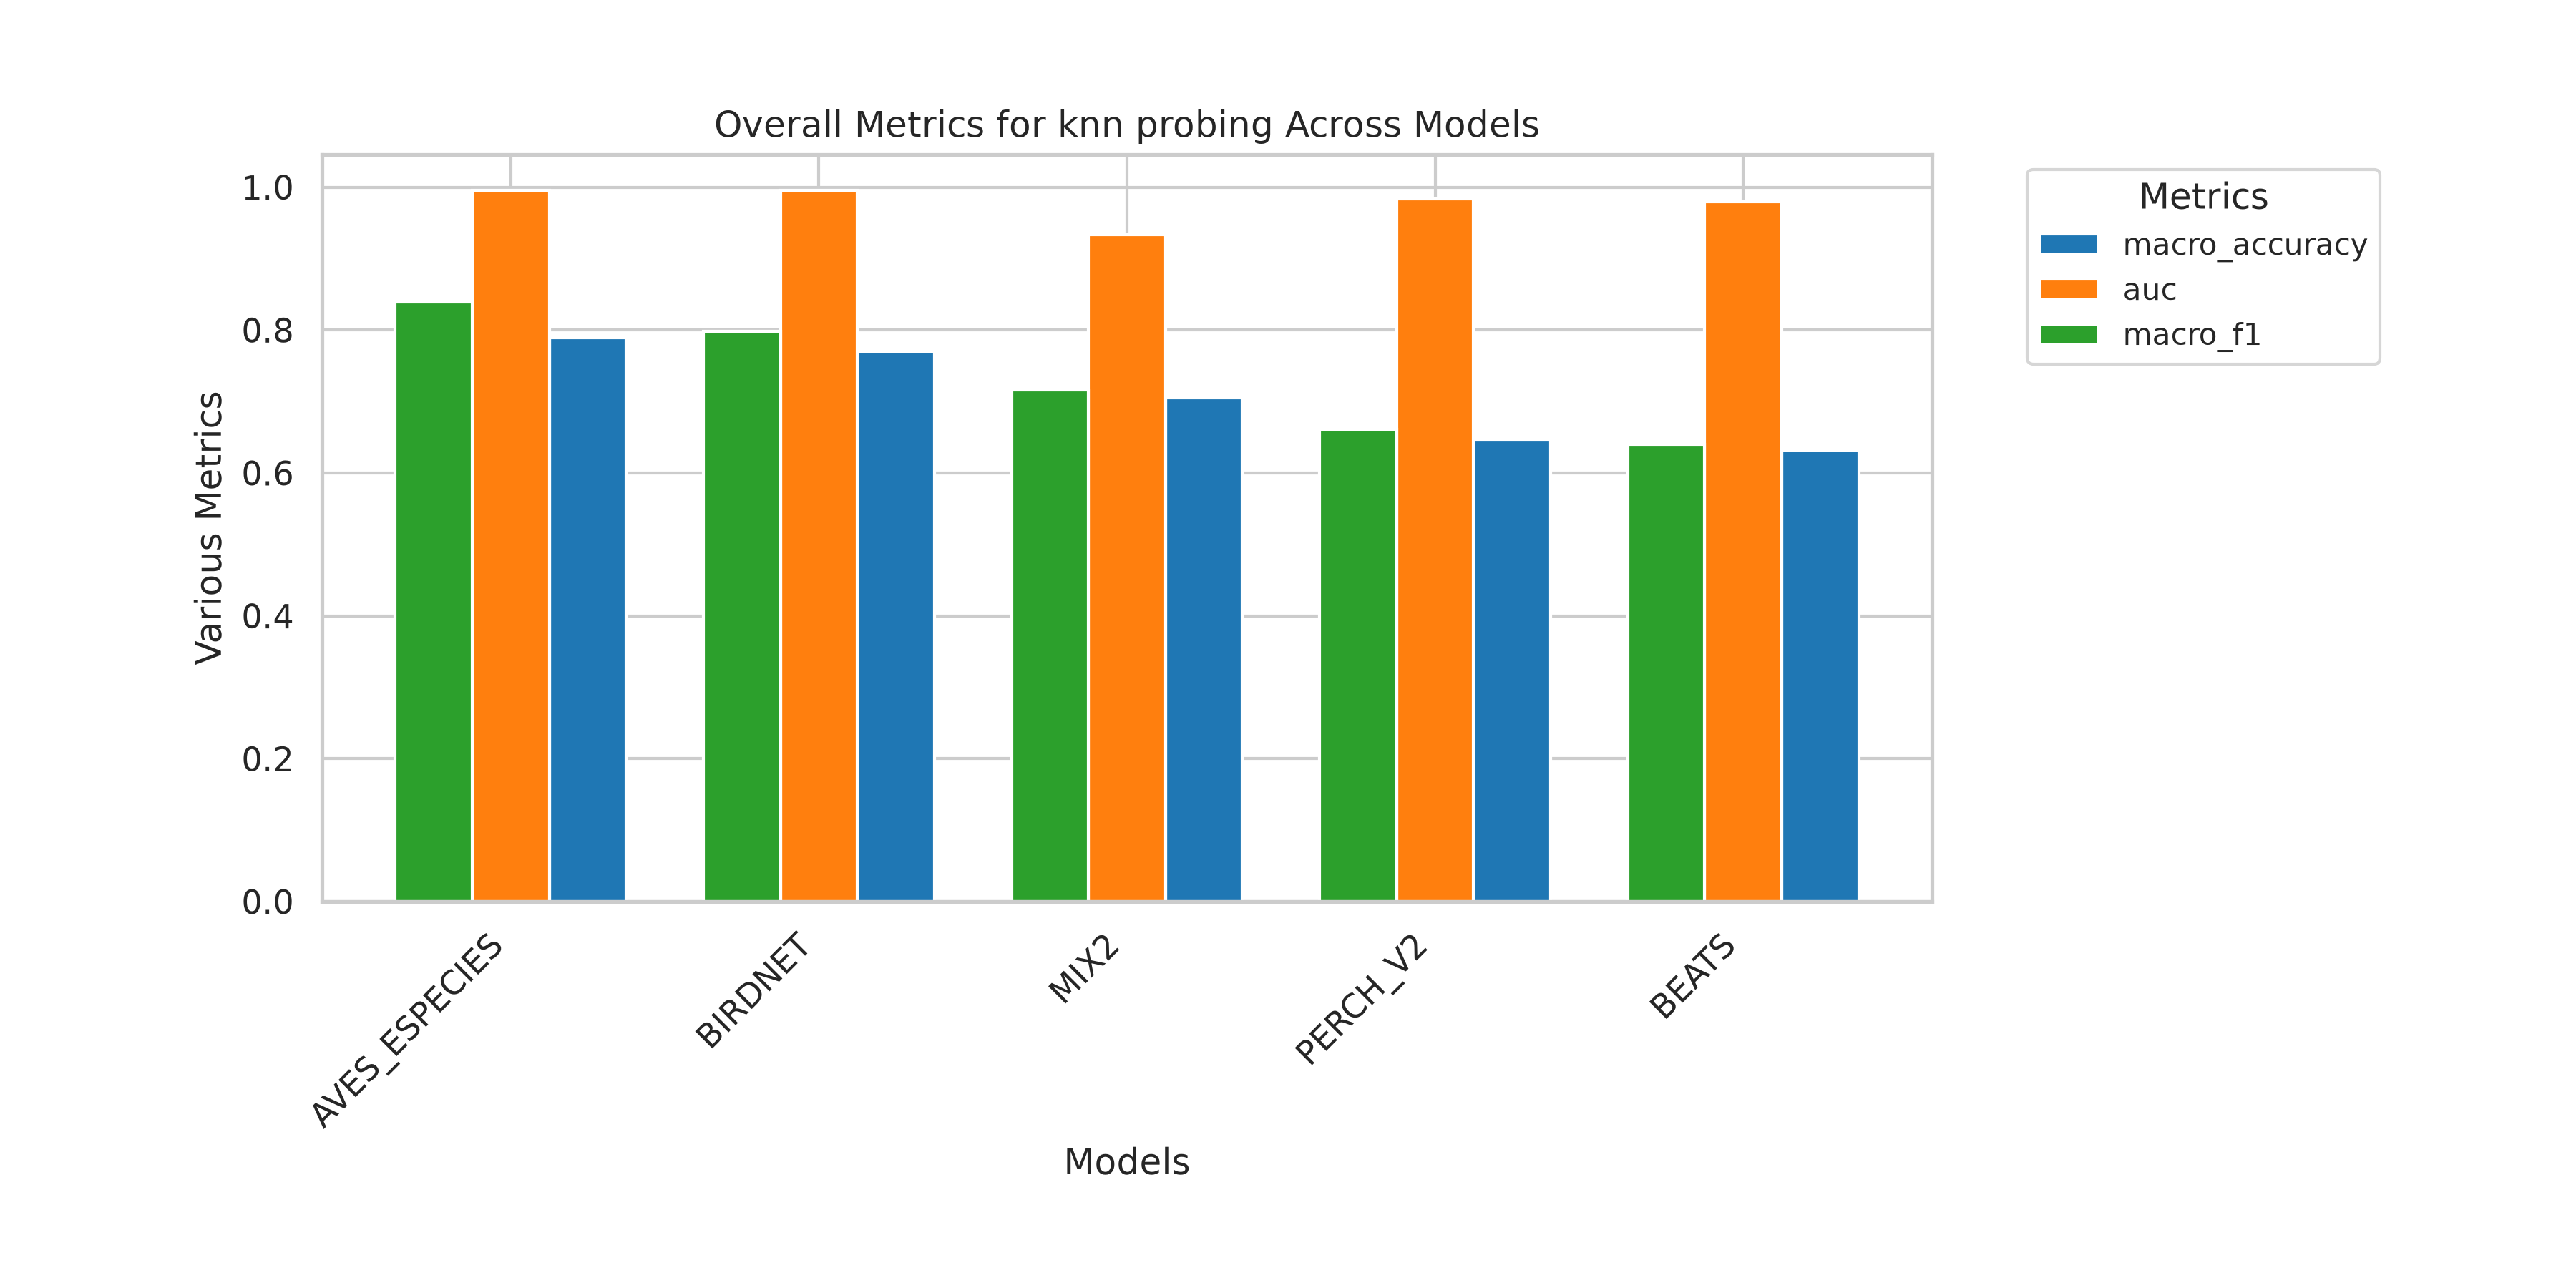
\includegraphics[width=\textwidth]{supplementary/Initial/overview/overview_metrics_knn_probing_av-bi-mi-pe-be.png}
    \caption{Overall Metrics}
\end{figure}
\begin{figure}
    \centering
    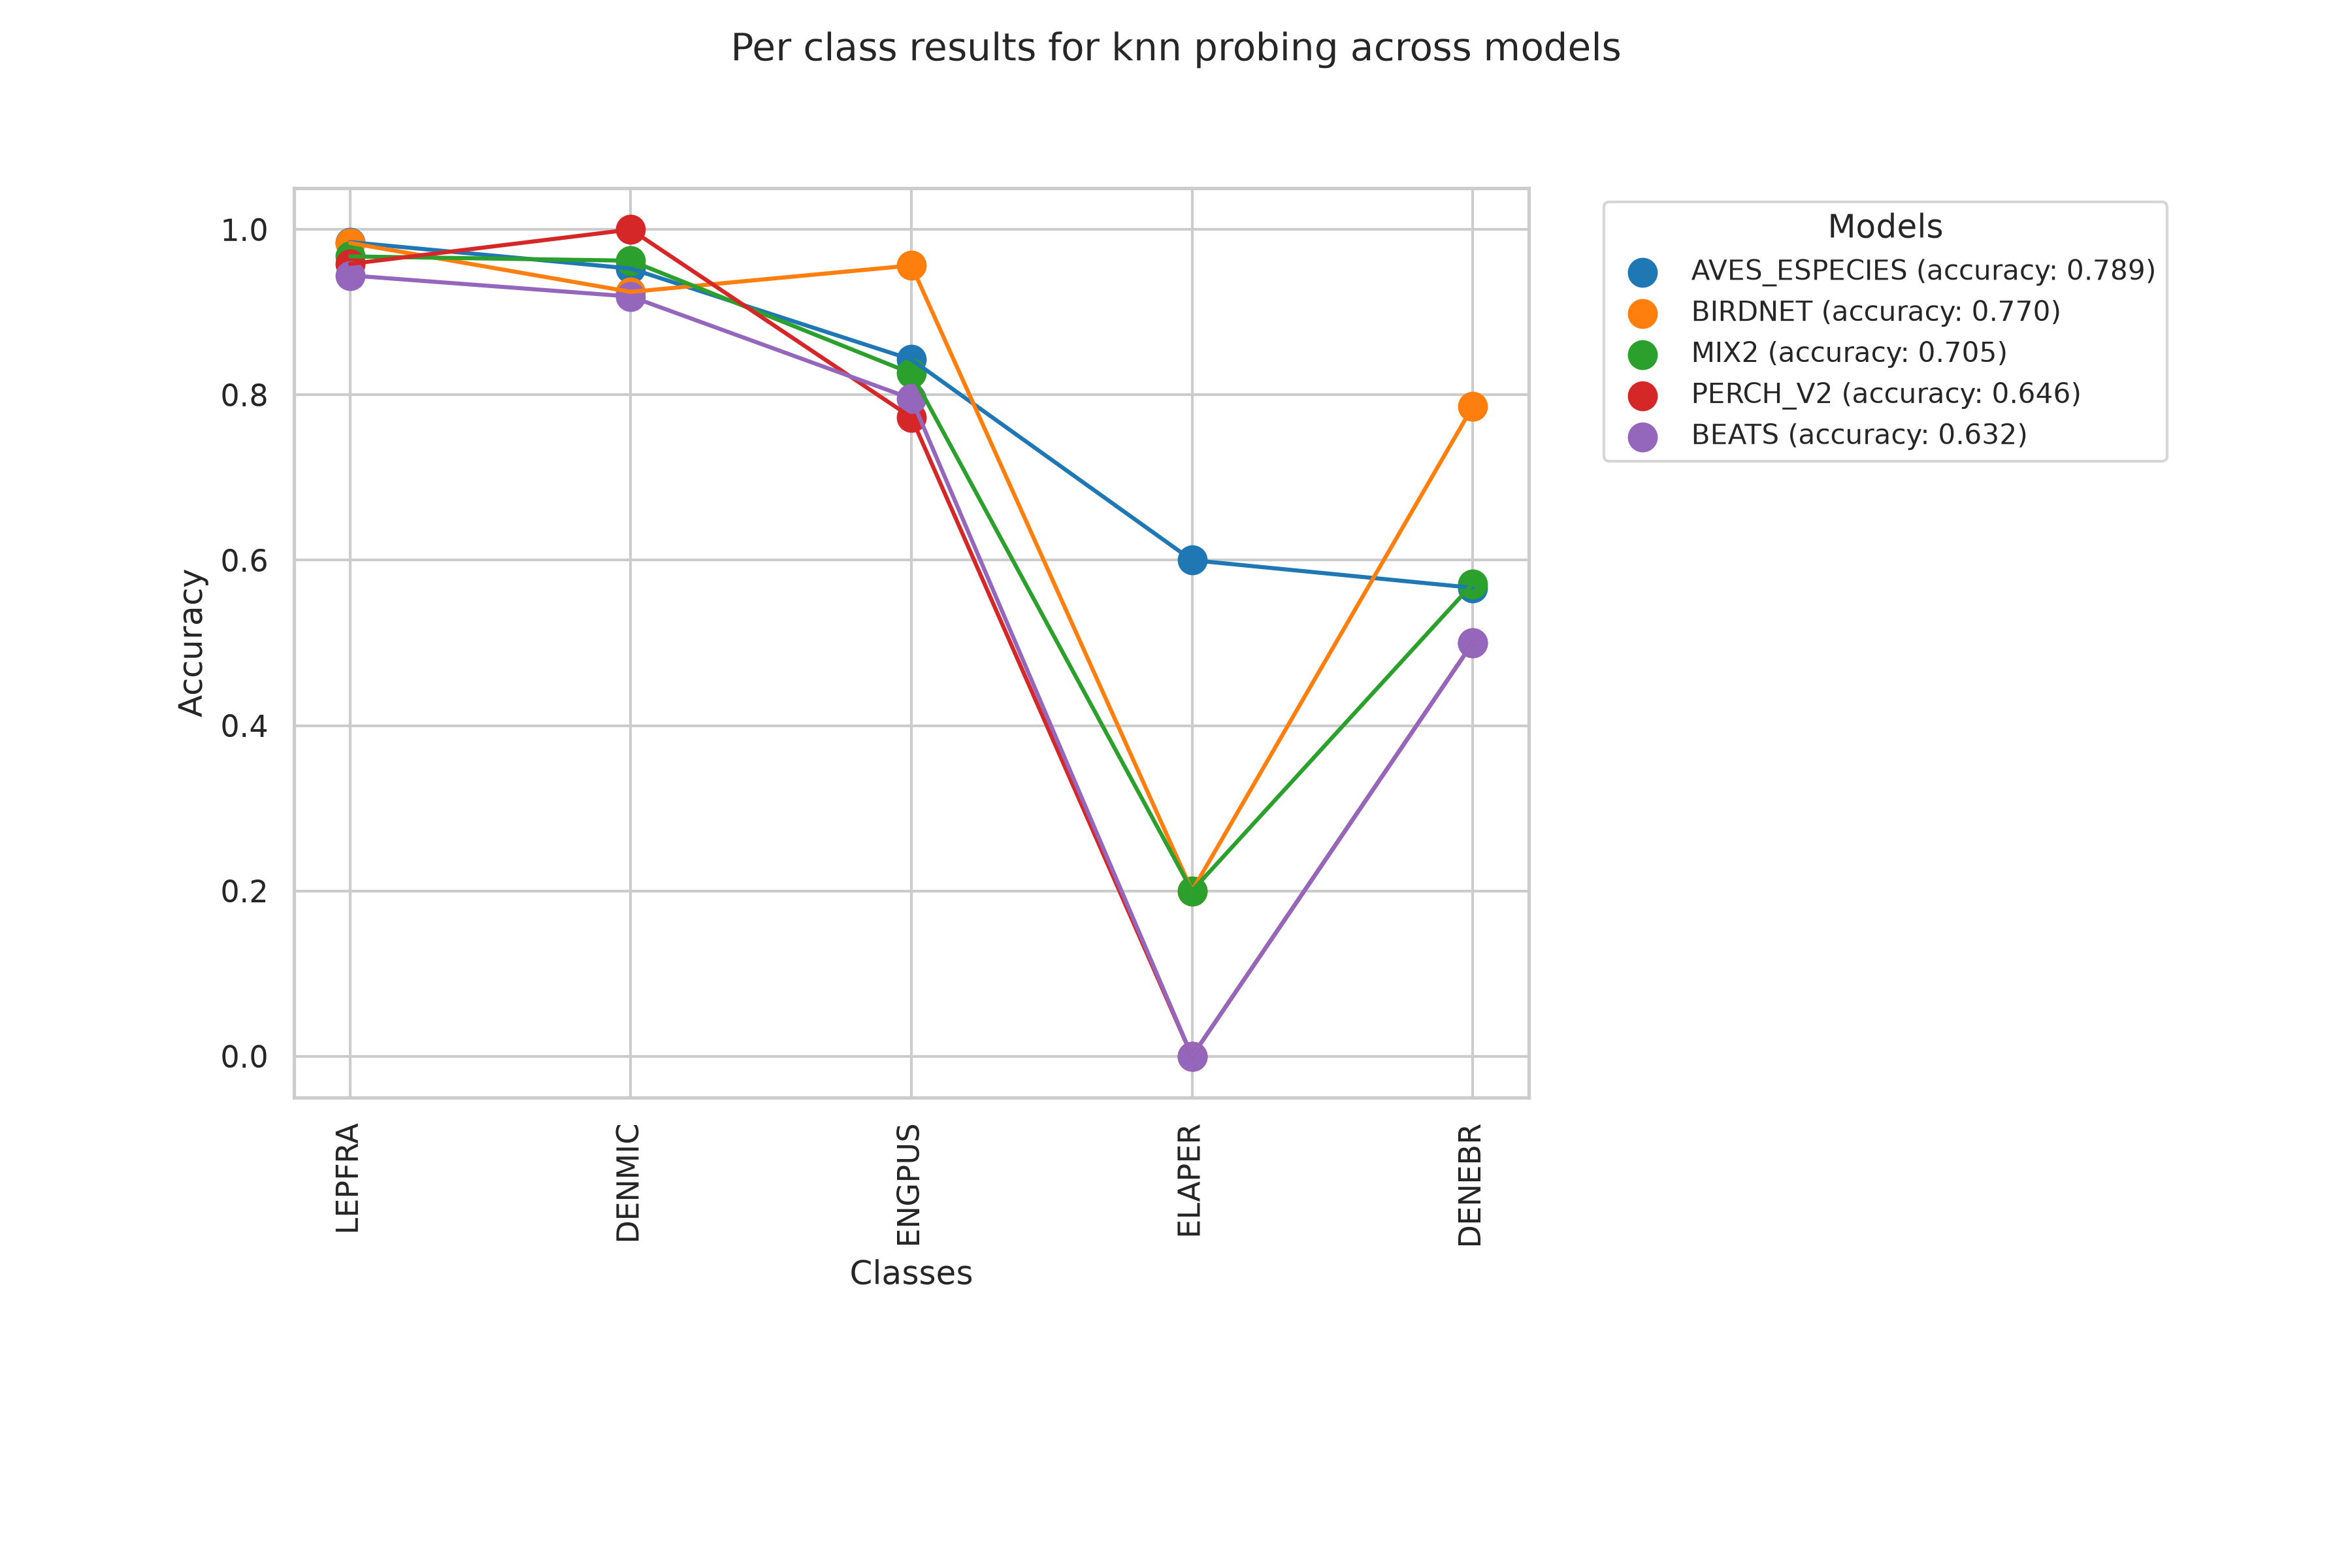
\includegraphics[width=\textwidth]{supplementary/Initial/overview/comparison_knn_probing_av-bi-mi-pe-be.png}
    \caption{Comparison per Class per Model}
\end{figure}
\begin{figure}
    \centering
    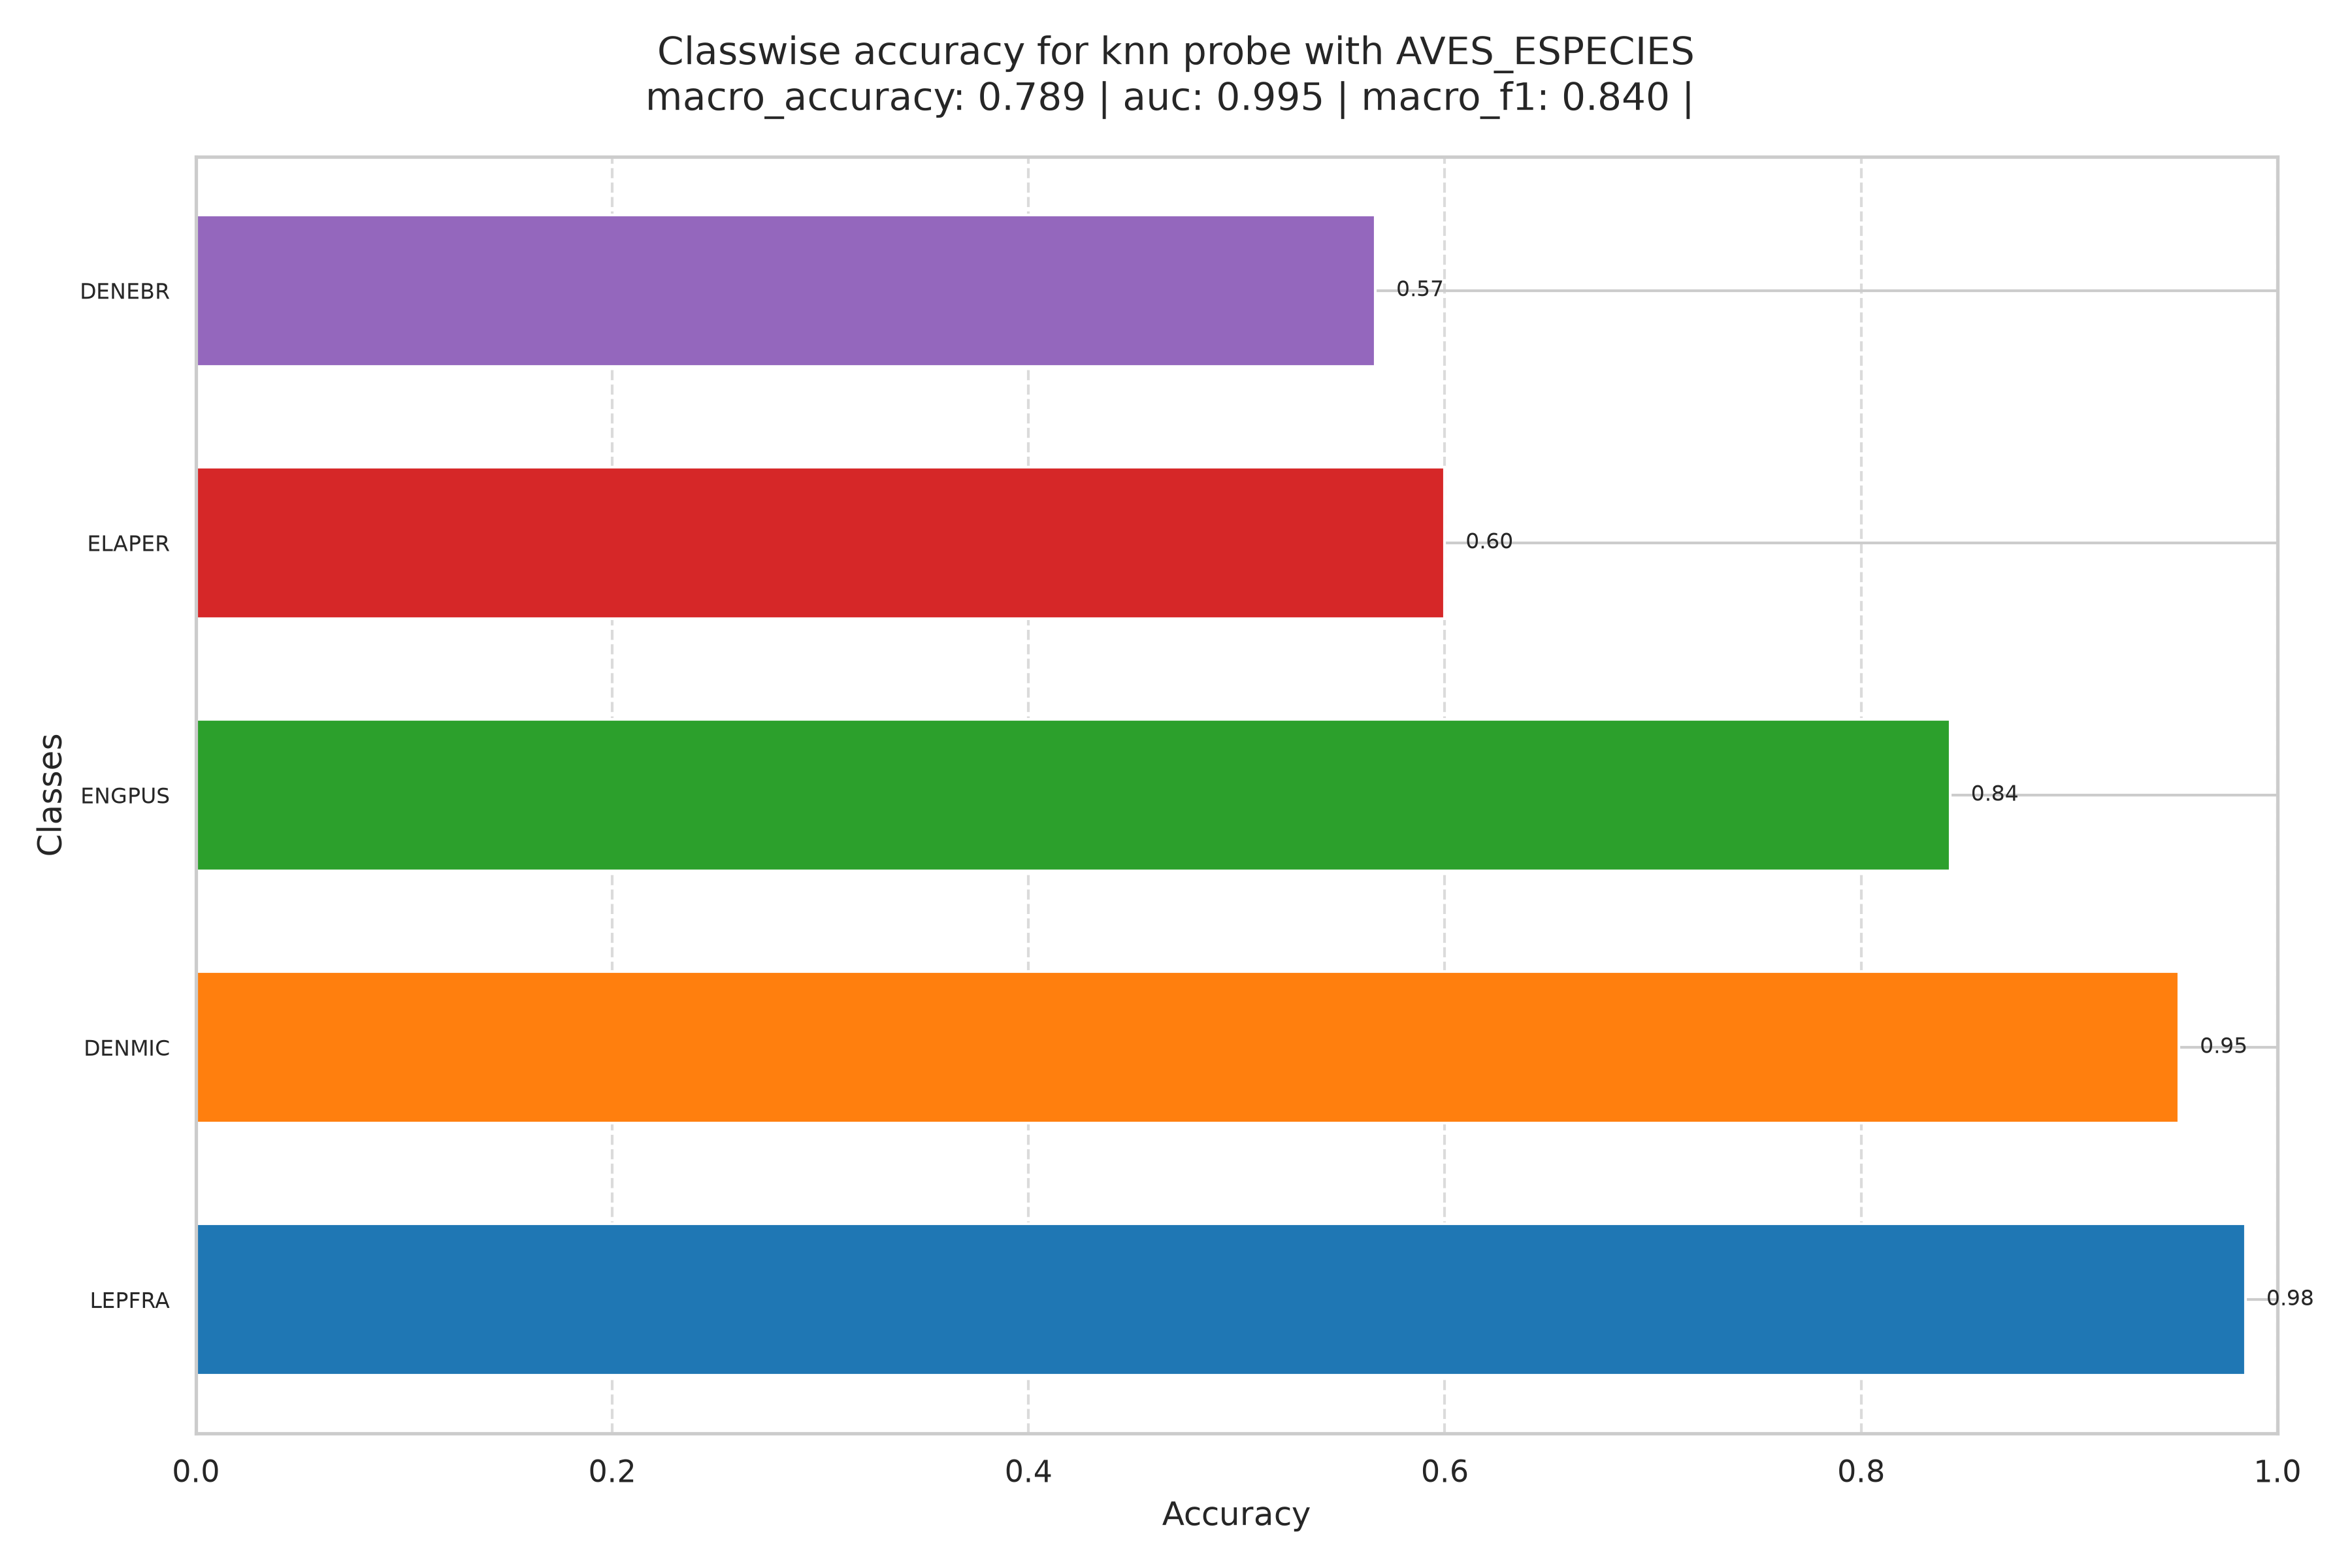
\includegraphics[width=\textwidth]{supplementary/Initial/aves_especies/plots/probe_results_knn_aves_especies.png}
    \caption{Aves Especies}
\end{figure}
\subsection{Classes vs. Performance}
Using \textit{bacpipe}, the Grillo and Silencio dataset were embedded and evaluated using the aves especies model. The hope was that increasing the training data, even with classes not of interest, would improve results for the classes of interest. The results were mixed. Some that had poor performance improved, but only to ~60 and the other classes dropped slightly. 
\begin{figure}
    \centering
    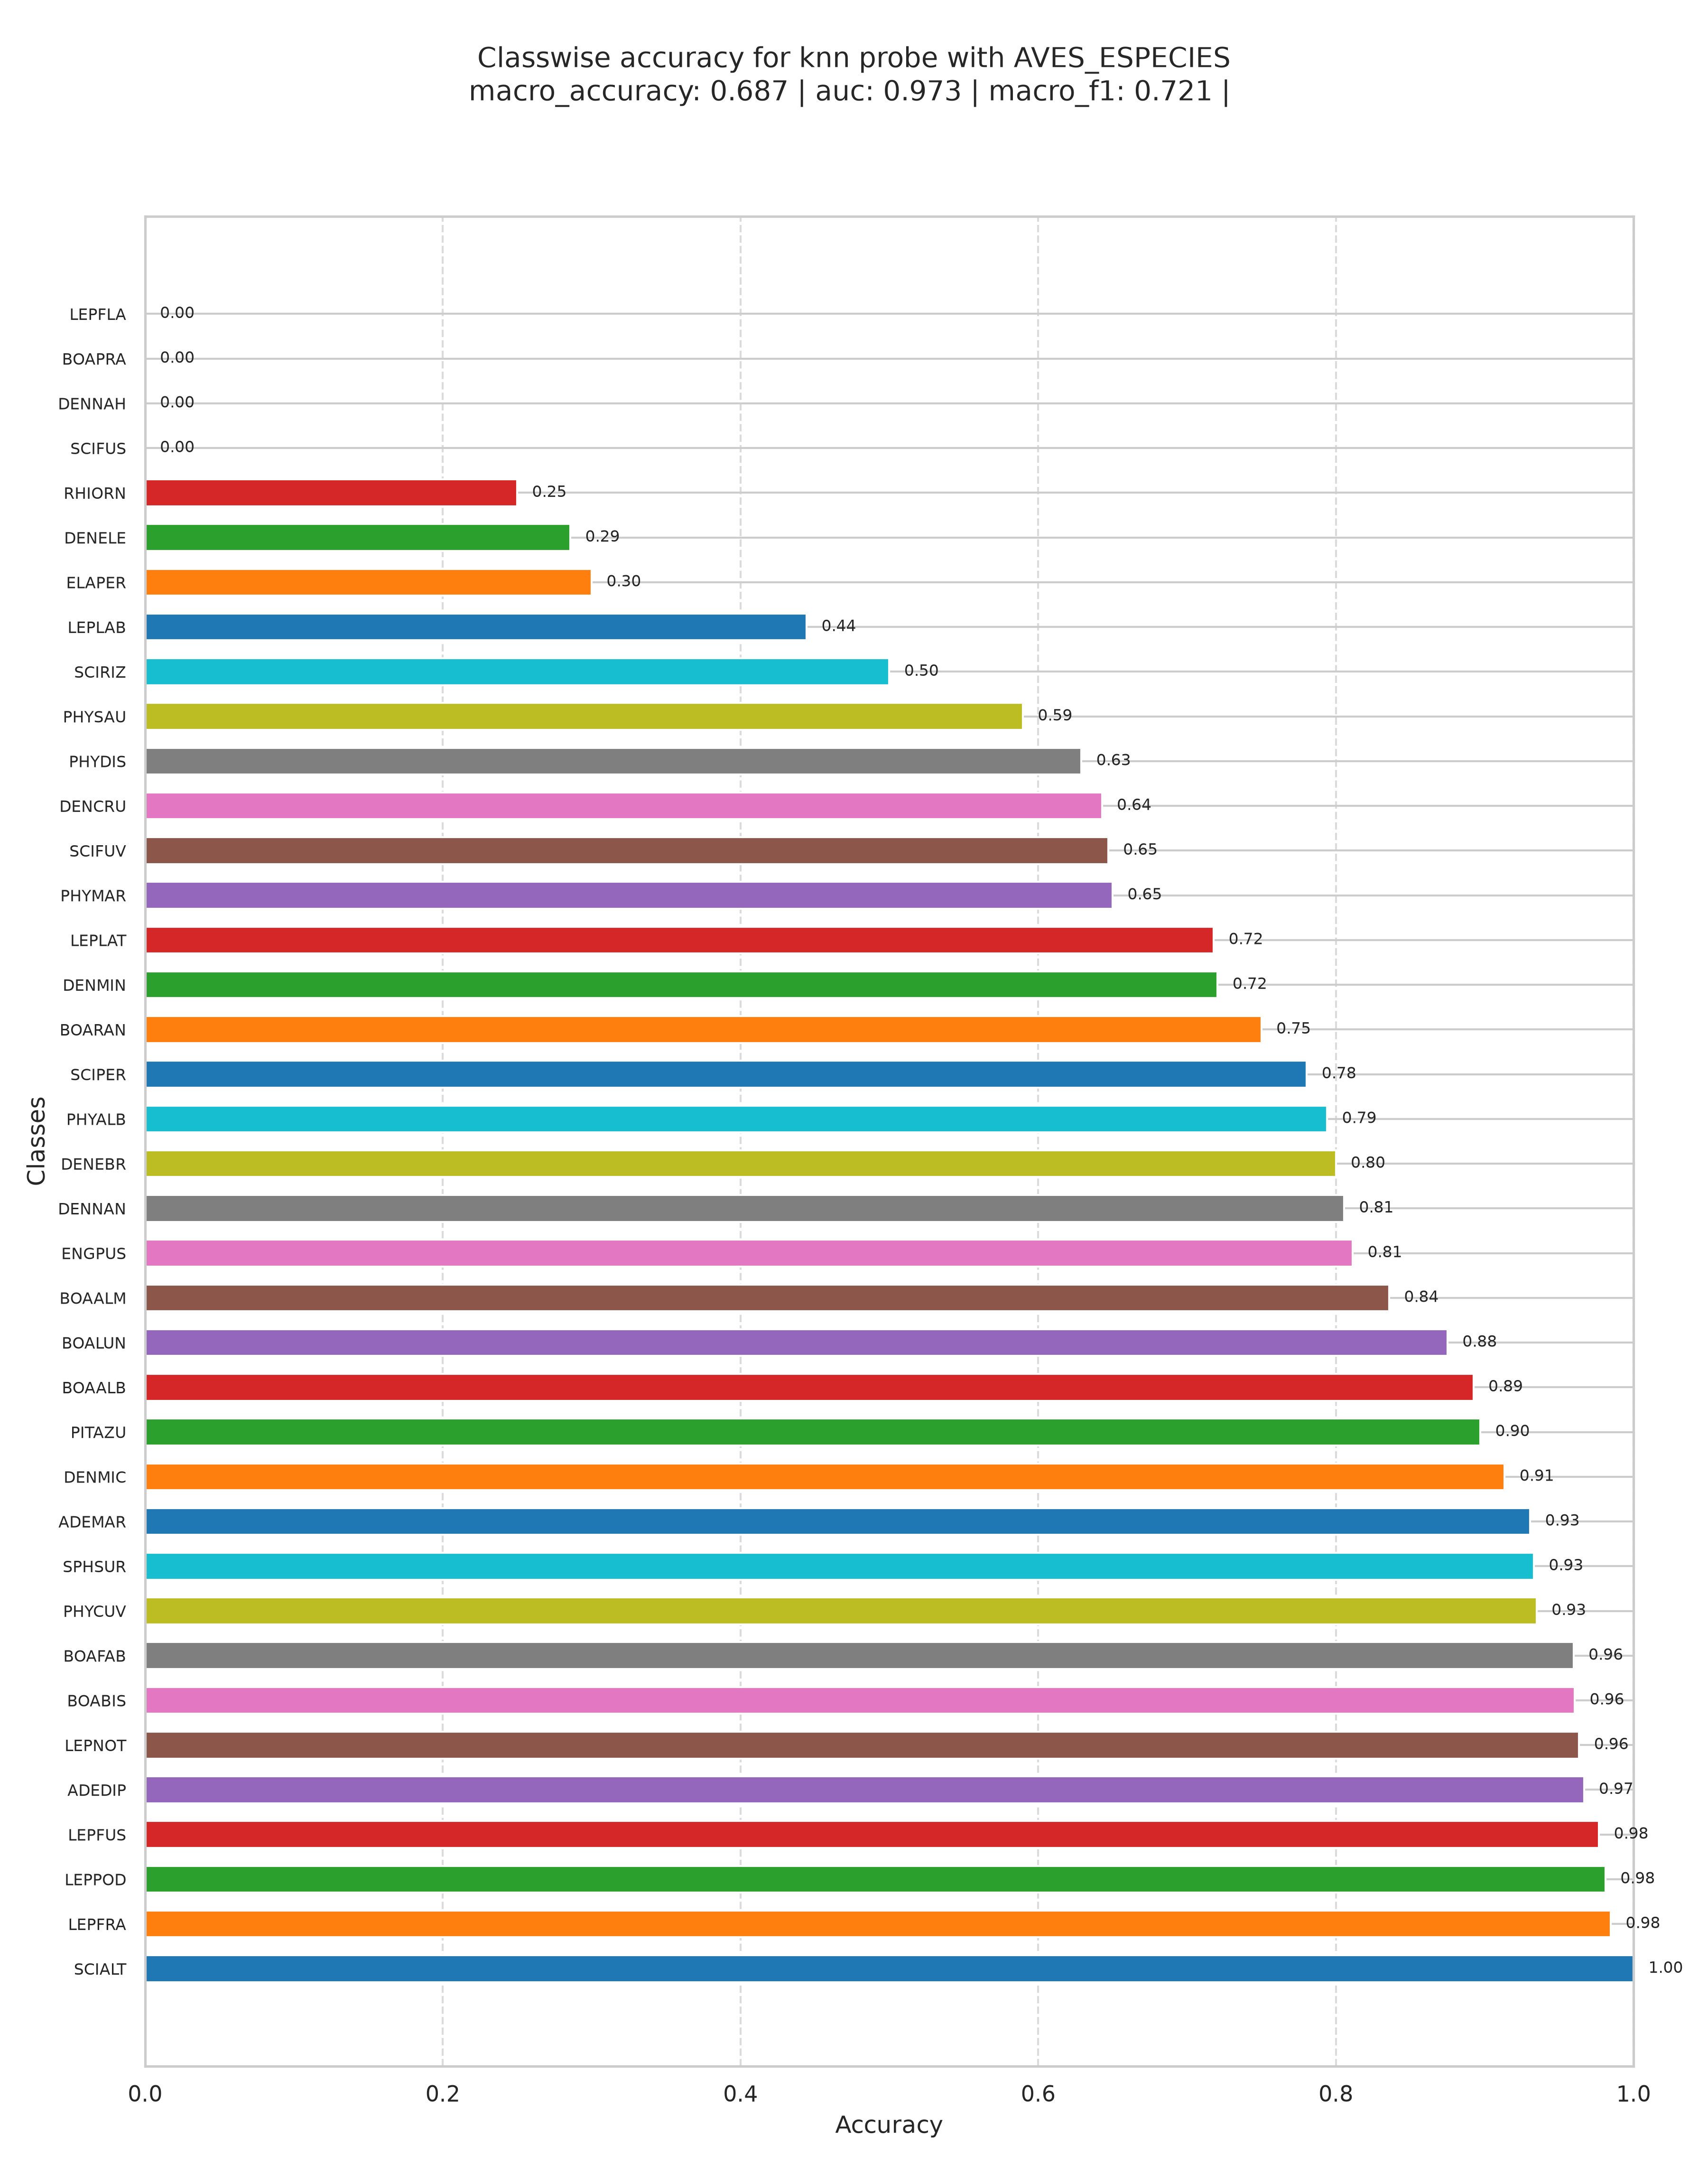
\includegraphics[width=\textwidth]{supplementary/IncreaseClasses/probe_results_knn_aves_especies.png}
    \caption{Increase of Classes}
\end{figure}
\subsection{AVEX}
Since we had the most success with Aves Especies, we decided to try the updated model Avex, which is a general classifier as opposed to a bird focused one (check paper, not sure). The results were comparabel with Aves Especies and BirdNet. Seeing as the support for some of these classes is so low, there is a noticeable stochastic effect between runs, and this time Birdnet had the highest AUC. 
\begin{figure}
    \centering
    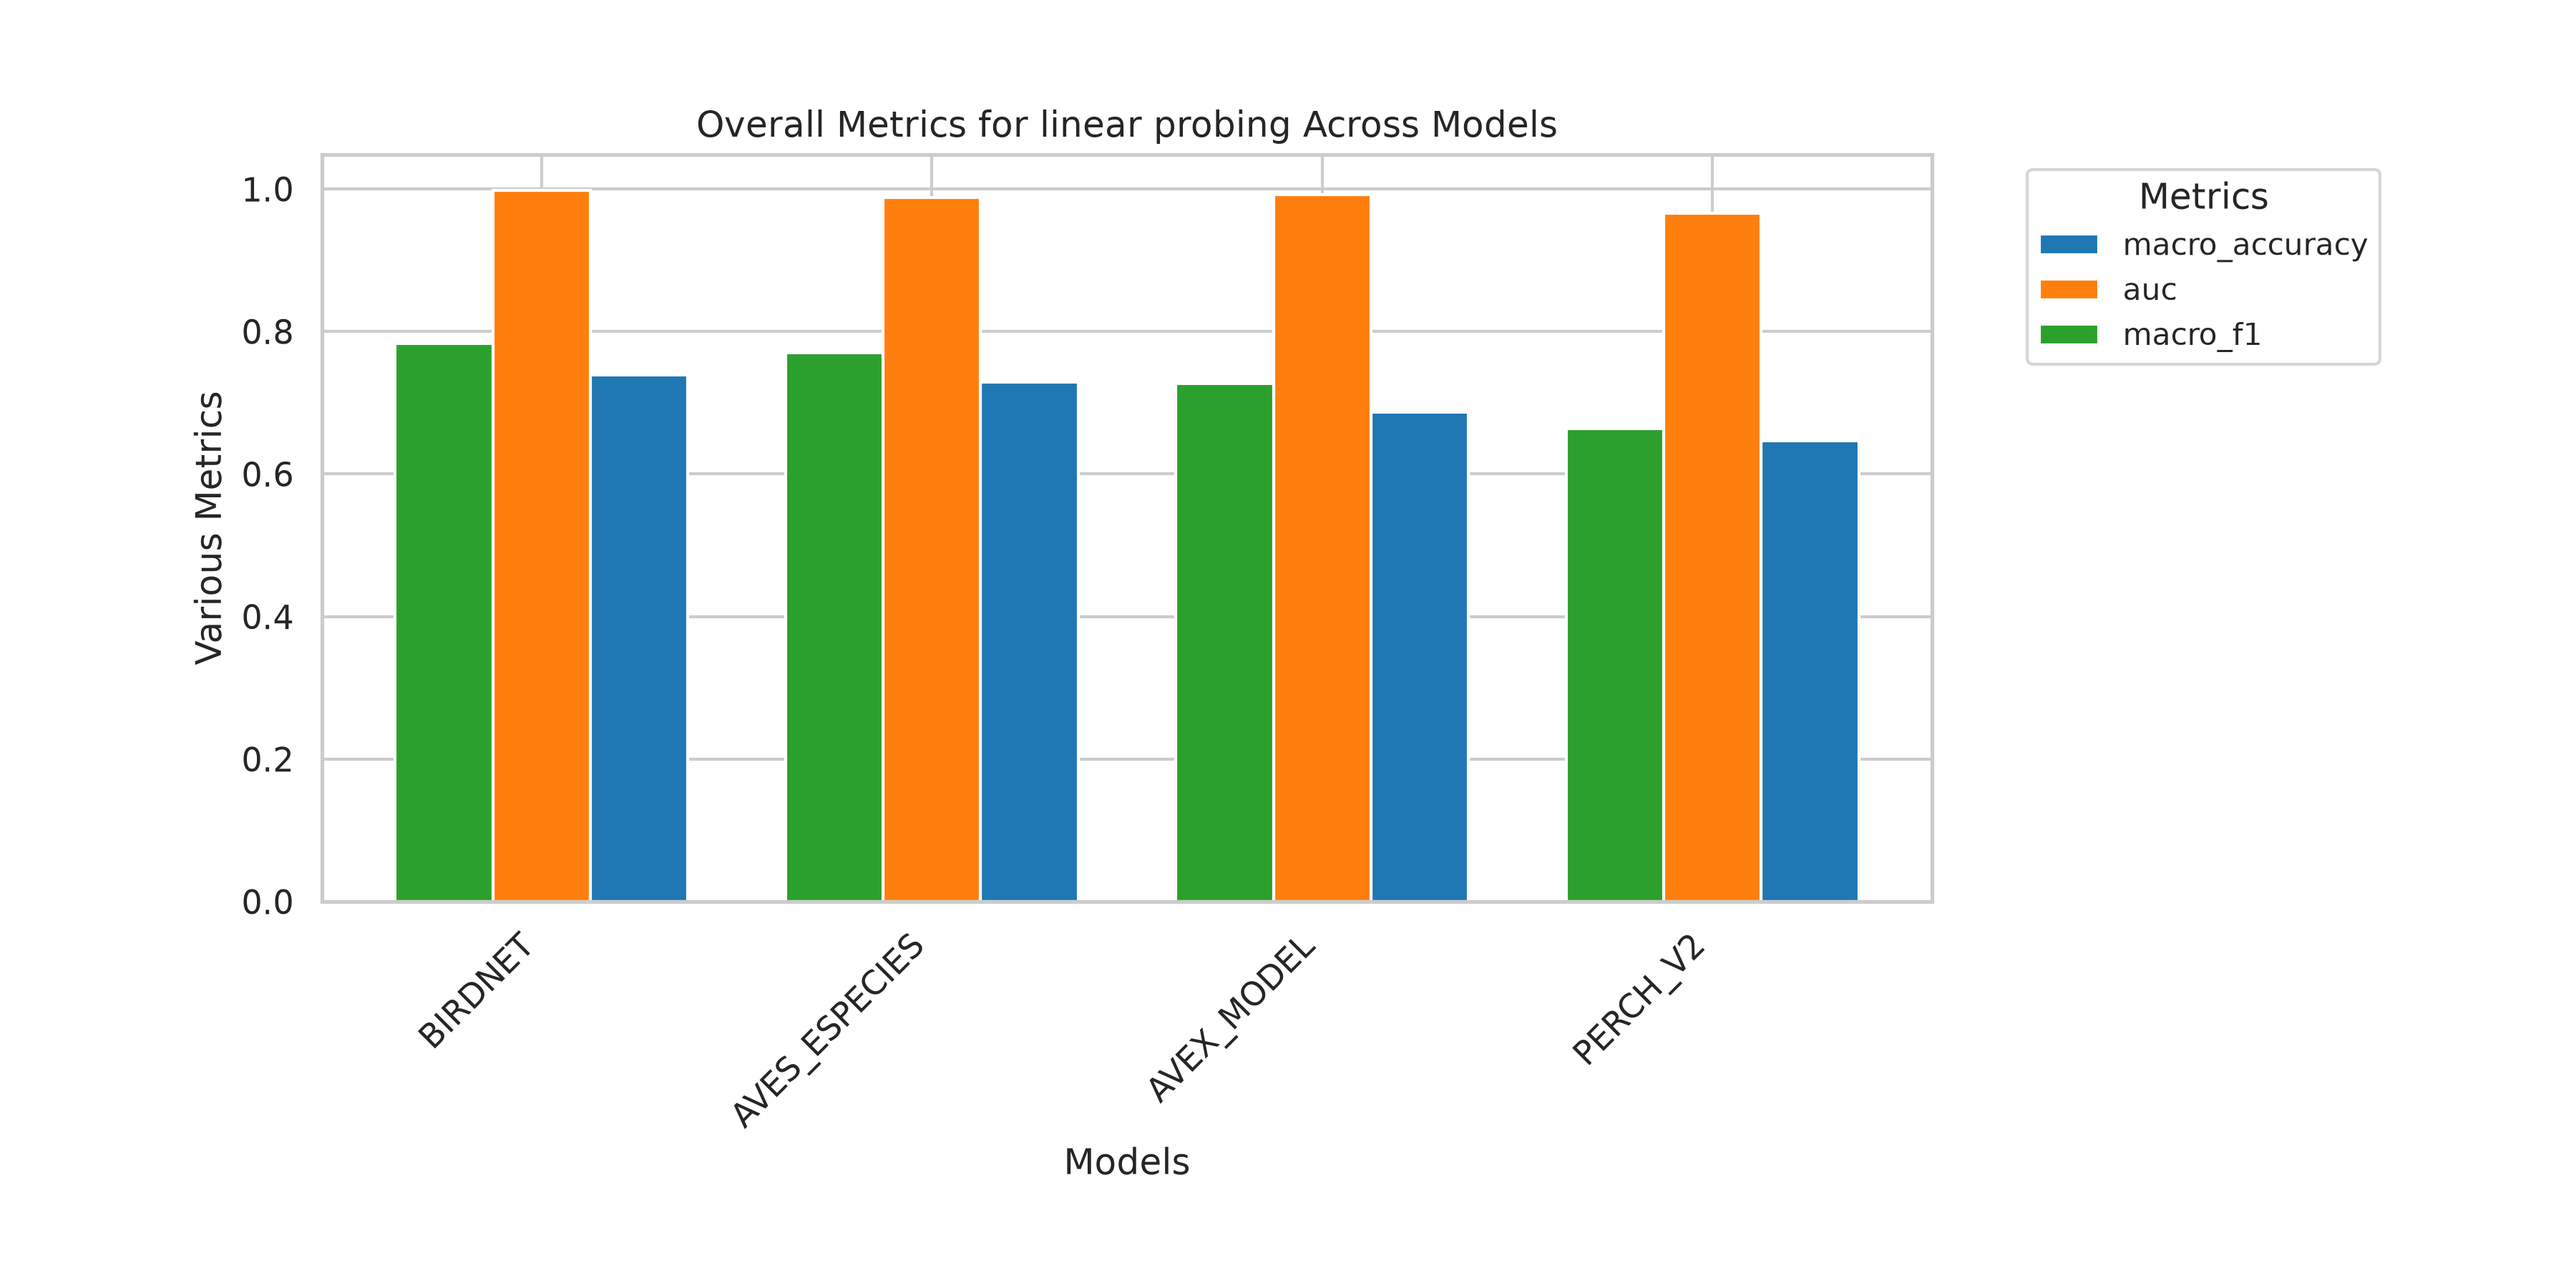
\includegraphics[width=\textwidth]{supplementary/Avex/overview_metrics_linear_probing_bi-av-av-pe.png}
\end{figure}
\subsection{PU-learning}
Positive-Unlabeled learning aims to utilize the mass amount of information that may be contained in the unlabeled portion of passive acoustic data. It mathematically corrects model predictions to (I believe) lessen the weight of learning a negative example. This biased negative weighting is already implemented in \textit{perch-hoplite}, and the ElkaNoto PU learning was implemented in bacpipe with less than promising results. However, the previous distribution $\pi$ was not estimated nor were other PU models tested. 

\cite{zhangMixupEmpiricalRisk2018, chenVariationalApproachLearning2020, yuanPositiveLabelAll2024} Novel PU approach that seems easy to follow/implement. Mixup could improve OOD-site generalization. 
\subsection{Hierarchy and Contrastive Learning}
Training a slighter larger, but still small, neural network on top of the frozen embeddings to learn hierarchical information. This could be phonic, as in first determining if a clip is biophonic, environmentalphonic, or anthrophonic, then determing species from there. Or, taxonomical, and learning the Family $\rightarrow$ Genus $\rightarrow$ Species relationships. The weighted contrastive loss function can preserve this relationship such that the probabilities at each taxonomic level sum to the levels higher.  

It seems that the best loss function / architecture is the FTM only from \cite{kuHierarchyAwareRepresentationLearning}. This is based off the Hierarchy metrics as found in \cite{kiritchenkoLearningEvaluationPresence2006}. 
\section{Annotations}
\subsection{spectrolipi}
Spectrolip is a web-based annotation platform that allows users to upload a custom species list and view and play audio files as spectrograms. The user then selects a species and subsequent bounding boxes are assigned that ID. This has been great for cold-start species, but progress is much slower than the active learning pipeline. 
\url{https://spectrolipi.com/}
\subsection{Active Learning}
Currently, the website serves example for annotation based on the logit score from the classifier. The windows are sorted by absolute distance from zero as this focuses annotation effort on the model's decision boundary. They are given in batches according to species, so that the user is given a batch of ~$k$ examples to review for $i$th specie. 
\[ unc(x) = \frac{1}{|\mathscr{S}|} \sum_{k \in \mathscr{S}} H(p_k(x)) \]
\[H(p) = -p\log p - (1-p)\log(1-p)\]
\textit{Diversity} is the distance from a snippet's embedding to its nearest labelled neighbour, encouraging coverage of underxplored regions of the embedding space. Specifically, it is the cosine distance to the nearest annotated neighbour. 

\textit{Density} is a $k$-nearest-neighbour density estimate within the unlabelled pool, down-weighting isolated outliers that are unlikely to be representative of the broader data distribution.\cite{gouveaYAPATOpenSourcePlatform2026} \cite{settlesActiveLearningLiterature, heActiveLearningApproach2014}


The composite score is defined in Figure 4. as 
\[w_1 \cdot unc + w_2 \cdot div + w_3 \cdot den\]
\[w_1 + w_2 + w_3 = 1\]

Another paper also used a composite score, but only with diversity and uncertainty \cite{kathLeveragingTransferLearning2024}. 


\cite{lindholmAggregationStrategiesEfficient2025} This could be a neat way to go from 5-second 'weak' annotations to 1-second windows / more accurate annotations. 

\subsection{Annotator Agreement}
" In other words,
given two coding schemes for the same phenomenon, the one with fewer categories will result
in higher percentage agreement just by chance." (page. 13 (statistical methods) \cite{artsteinInterCoderAgreementComputational2008})


\section{Website}
Just as their exists limited resources on anuran datasets, there doesn't exist a uniform platform to be able to learn frog calls. So, we created the OsaAnuran website to be a place where people can learn the frog calls of the amphibians on the Osa Peninusla. The primary page displays 12 of the 52 species. Each species is displayed on a card that contains their scientific name, a photo, and various audio samples. The card contains a button that can be clicked to display more information about a species, such as its habitat, IUCN status, range, and endemism. 

There is Learn section to the website that displays a random audio from the main page and asks user to choose the correct species out of four possible answers. A correct answer earns 10 points and an incorrect answer takes away 10 points. This could be a great 'onboarding' for new volunteers interested in helping the annotation effort. 
\url{https://osaconservation.github.io/OsaAnurans/}

\section{Updates}
\subsection{2026-09-23}
First, I downloaded available .wav files for 42 of the 52 anuran species from GBIF.
Then, I started to build a machine learning workflow using Anuraset. I have implemented preprocessing, embedding, and classifier scripts. I am now learning about Positive Unlabeled and Multiple Instance Learning techniques to improve classifier performance.

\subsection{2026-10-28}
This month progress was made across three fronts of the project: annotation, embedding generation, and classifier training. 

An annotation protocol was developed using the OsaAnurans website, hosted on github, as well as spectrolipi, an online annotation platform. 
Multiple sessions were run with volunteers and fellows, and 5 recordings were annotated completely. 
These recordings mainly contained calls of \emph{Dendropsophus ebbracatus} and \textit{Scinax boulengeri}. 
Additionally, a new annotation workflow has been developed and will be tested with live volunteers in the following days. 
This new protocol takes advantage of the embedding hyperspace to allow for a similarity search to be ran over many hours of recordings, and hopefully quicken annotation generation and increase general accuracy. 

Embedding generation is currently being done through \textit{bacpipe}, a python package that allows for quick comparison between many different off-the-shelf models. 
We found that \textit{aves especies} had the best clustering and separation compared to more robust models like \textit{perchV2} and \textit{BirdNetV2}. 
The next step will be to connect the \textit{bacpipe} workflow to a \textit{perch-hoplite database} that will allow for quicker comparison searches as well as improved transferability between machines. 

The \textit{Silencio} dataset was filtered to include only anuran species that are found here on the Osa Peninsula. 
With these five species, we were able to get a preliminary look at the separability and classification results for a future classifier. 
The model had an average accuracy of 0.807, an AUC of 0.996, and an average f1 score of 0.852.
These results look quite promising, but it must be remembered the setting that they were generated in. 
These examples were taken from a curated dataset of Colombian species, and as such likely overestimate the results of field deployment of the model in Osa. 

\section{Motus Towers}
There seem to be four ways to connect to a Motus tower and download data: USB, FileZilla, SSH, and WIFI/local website.
\subsection{Sierpe}
Attempted to connnect via USB, but that failed. I was able to connect via FileZilla with the following credentials:
\begin{center}
    \begin{tabular}{c c}
    Host: & sftp://sensorstation.local \\
    Username: & ctt \\
    Password: & ctt-station 
\end{tabular}
\end{center}
I was connected via Ethernet at the time. 
I also connected via SSH, which allowed for deleting the files on the Motus. 

\begin{center}
    \begin{tabular}{c c}
      ssh address: & ctt@169.254.130.47 \\
      ssh password: & ctt-station   
    \end{tabular}
\end{center}
The website download buttons did not work.

\subsection{Highlands}
None of the three previous attempts worked, especially considering there was no USB port / LCD menu. 
The sensorgnome was giving off a WIFI signal that I was able to connect to, and subsequently download that data from the web interface, although the download all button did not work. 
\begin{center}
    \begin{tabular}{c c}
        IP address: & 192.168.7.2 \\
        ssh password: & Unknown
    \end{tabular}
\end{center}
\begin{center}
    \begin{tabular}{c c}
        WIFI: & SG-39B8RPI36A4A \\
        Password: & sensorgnome-1 \\
        Website: & http://192.168.7.2:88/
    \end{tabular}
\end{center}

\subsection{Canopy Tower}
\begin{center}
    \begin{tabular}{c c}
        IP address: & 169.254.196.15 \\
        ssh password: & ctt-station
    \end{tabular}
\end{center}

\begin{center}
    \begin{tabular}{c}
        scp -r ctt@169.254.196.15:/data .
    \end{tabular}
\end{center}

\printbibliography
\end{document}